%\documentclass[%
	%draft
%	]{ijsra}
\def\IJSRAidentifier{\currfilebase} %<---- don’t change this!
%-------Title | Email | Keywords | Abstract-------------
\def\maintitle{A Reassessment of Natufian Sedentism}
\def\shorttitle{\maintitle}
\def\cmail{sgyn3538@uni.sydney.edu.au}
\def\keywords{Near Eastern Archaeology, Natufian, Settlement Dynamics, Mobility and Sedentism}

%\def\keywordname{}%<--- redefine the name “Keywords“ in needed language
\def\abstract{The Natufian assemblage (ca. \num{13000}–\num{10300} years BP) in the Levant has largely been understood to reflect sedentary communities. However, thorough analysis of the material has demonstrated that a misunderstanding of sedentism and misinterpretations of cultural material have driven this claim. Scholars including Edwards and Shewan have significantly contributed to the debate and convincingly argued for Natufian mobility. This literature review summarises early thought and study of Natufian sites and identifies the strengths and weaknesses. It then discusses more recent research and opinions that challenge long held notions of Natufian sedentism. The Natufian assemblage represents a key period in the history of human behaviour, and consequently, a comprehensive and rigorous analysis of the Natufian assemblage is important for understanding the transition from mobile to sedentary communities, and the material culture that results. A review and consideration of the various aspects of the debate is necessary for continuing further research.}
%--------Author’s names------------
\def\authorone{Sarah Gyngell}
%-------Biographical information-------------
\def\bioone{Sarah is an undergraduate student at the University of Sydney where she is completing a Bachelor of Arts and Science majoring in Archaeology and Marine Science. She plans to study Epipaleolithic Near Eastern Archaeology for her Honours, with a focus on changing settlement dynamics during the mobile to sedentary transition. Sarah hopes to apply her background in geoscience and the use of GIS to contribute to future research. She has field experience in Jordan, where she was a volunteer at Pella in 2015. Sarah has also worked at a historic site in Sydney and volunteered for numerous organisations and events including the 2015 Australian National Archaeology Student Conference.}
%------University/Institution--------------
\def\affilone{Department of Archaeology, University of Sydney}

\begin{filecontents}{\IJSRAidentifier.bib}
%Bibliography-data HERE
@incollection{Bar-Yosef_1983,
	author = {Bar-Yosef, O.},
	editor = {Young, T. and Smith, P. and Mortensen, P.},
	title = {The Natufian in the Southern Levant},
	booktitle = {The Hilly Flanks and Beyond: Essays on the Prehistory of 	Southwestern Asia},
	date = {1983},
	pages = {11--42},
	publisher = {The Oriental Institute of the University of Chicago},
	location = {Chicago},
}

@article{Bar-Yosef_1998,
	author = {Bar-Yosef, O.},
	title = {The Natufian Culture in the Levant, Threshold to the Origins of 	Agriculture},
	journaltitle = {Evolutionary Anthropology},
	date = {1998},
	pages = {159-–177},
	volume = {6},
}

@article{Bar-Yosef_2011,
	author = {Bar-Yosef, O.},
	title = {Climatic Fluctuations and Early Farming in West and East Asia},
	journaltitle = {Current Anthropology},
	date = {2011},
	pages = {S175--S193},
	volume = {52},
	series= {4},
}



@incollection{Fletcher_1998,
author = {Fletcher, R.},
title = {African Urbanism},
subtitle = {Scale, Mobility and Tranformations},
editor = {Connah, G.},
booktitle = {Transformations in Africa},
pages = {104-138},
year = {1998},
location = {London},
publisher = {Leicester University Press},
}


@article{Bar-Yosef_1989,
	author = {Bar-Yosef, O. and Belfer-Cohen, A.},
	title = {The Origins of Sedentism and Farming Communities in the Levant},
	journaltitle = {Journal of World Prehistory},
	date = {1989},
	pages = {447--498},
	volume = {3},
	issue = {4},
}

@incollection{Bar-Yosef_1991,
	author = {Bar-Yosef, O. and Valla, R.},
	editor = {Bar-Yosef, O. and Valla, R.},
	title = {The Natufian Culture: An Introduction},
	booktitle = {The Natufian Culture in the Levant},
	date = {1991},
	pages = {1--10},
	publisher = {International 	Monographs in Prehistory},
	location = {Michigan},
}

@article{Belfer-Cohen_1991,
	author = {Belfer-Cohen, A.},
	title = {The Natufian in the Levant},
	journaltitle = {Annual Review of Anthropology},
	date = {1991},
	volume = {20},
	pages = {167--186},
}

@incollection{Belfer-Cohen_2013,
	author = {Belfer-Cohen, A. and Goring-Morris, A.},
	editor = {Bar-Yosef, O. and Valla, F.},
	title = {Breaking the Mould: Phases and Facies in the 	Natufian of the Mediterranean Zone},
	booktitle = {Natufian 	Foragers in the Levant: Terminal Pleistocene Social Changes in Western Asia},
	date = {2013},
	pages = {544--561},
	publisher = {International 	Monographs in Prehistory},
	location = {Michigan},
}

@book{Byrd_2005,
	author = {Byrd, B.},
	title = {Early Village Life at Beidha, Jordan: Neolithic Spatial Organisation and Vernacular Architecture},
	date = {2005},
	publisher = {Oxford University Press},
	location = {New York},
}

@article{Boyd_2006,
	author = {Boyd, B.},
	title = {On ‘sedentism’ in the Later Epipalaeolithic (Natufian) Levant},
	journaltitle = {World Archaeology},
	date = {2006},
	volume = {38},
	issue = {2},
	pages = {164--178},
}

@book{Childe_1953,
	author = {Childe, V.},
	title = {New Light on the Most Ancient Near East},
	date = {1953},
	publisher = {Praeger},
	location = {New York},
}

@article{Edwards_1989,
	author = {Edwards, P. C.},
	title = {Problems of recognising earliest sedentism: the Natufian example},
	journaltitle = {Journal of Mediterranean Archaeology},
	date = {1989},
	volume = {2},
	pages = {5--48},
}

@book{Edwards_2013,
	author = {Edwards, P. C.},
	title = {Wadi Hammeh 27, an Early Natufian Settlement at Pella in Jordan},
	date = {2013},
	publisher = {Brill},
	location = {Leiden},
}

@article{Edwards_2015,
	author = {Edwards, P. C.},
	title = {Natufian interactions along the Jordan Valley},
	journaltitle = {Palestine Exploration Quarterly},
	date = {2015},
	volume = {4},
	issue = {147},
	pages = {272--282},
}

@article{Finlayson_2013,
	author = {Finlayson, B.},
	title = {Imposing the Neolithic on the past},
	journaltitle = {Levant},
	date = {2013},
	volume = {45},
	issue = {2},
	pages = {133--148},
}


@book{Fletcher_2007,
	author = {Fletcher, R.},
	title = {The Limits of Settlement Growth: A Theoretical Outline},
	date = {2007},
	publisher = {Cambridge University Press},
	location = {Cambridge},
}

@article{Garrod_1957,
	author = {Garrod, D.},
	title = {The Natufian culture: the life and economy of a Mesolithic people in the Near East},
	journaltitle = {Proceedings of the British Academy},
	date = {1957},
	issue = {43},
	pages = {211--227},
}

@article{Habu_1996,
	author = {Habu, J.},
	title = {Jomon sedentism and intersite variability: collectors of the Early Jomon Moroiso Phase in Japan},
	journaltitle = {Arctic Anthropology},
	date = {1996},
	volume = {33},
	issue = {2},
	pages = {38--49},
}

@article{Hardy-Smith_2004,
	author = {Hardy-Smith, T. and Edwards, P. C.},
	title = {The garbage crisis in prehistory: artefact discard patterns at the Early Natufian site of Wadi Hammeh 27 and the origins of household refuse disposal strategies},
	journaltitle = {Journal of Anthropological Archaeology},
	date = {2004},
	issue = {23},
	pages = {253–-289},
}

@incollection{Lieberman_1999,
	author = {Lieberman, D.},
	editor = {Rocek, T. and Bar-Yosef, O.},
	title = {Natufian “Sedentism” and the Importance of Biological Data for 	Estimating Reduced Mobility},
	booktitle = {Seasonality and Sedentism: Archaeological Perspectives from Old and New World Sites},
	date = {1999},
	publisher = {Peabody Museum of Archaeology and Ethnology},
	location = {Harvard University},
	pages = {75--92},
}

@book{Parslow_2009,
	author = {Parslow, C.},
	title = {Social Interaction in the Prehistoric Natufian: Generating an interactive agency model using GIS},
	date = {2009},
	publisher = {Archaeopress},
	location = {Oxford},	
}

@incollection{Shewan_2004,
	author = {Shewan, L.},
	editor = {Delage, C.},
	title = {Natufian Settlement Systems and Adaptive Strategies: The Issue of Sedentism and the Potential of Strontium Isotope Analysis},
	booktitle = {The Last Hunter-Gatherer Societies in the Near East},
	date = {2004},
	publisher = {John and Erica Hedges},
	location = {Oxford},
	pages = {55--94},
}

@article{Stutz_2002,
	author = {Stutz, A.},
	title = {Polarizing microscopy identification of chemical diagenesis in 	archaeological cementum},
	date = {2002},
	journaltitle = {Journal of Archaeological Science},
	issue = {29},
	year = {2002},
	pages = {1327–-1347},
}

@incollection{Tchernov_1991,
	author = {Tchernov, E.},
	editor = {Bar-Yosef, O. and Valla, F.},
	title = {Biological evidence for human sedentism in southwest Asia during 	the Natufian},
	booktitle = {The Natufian Culture in the Levant},
	date = {1991},
	pages = {315–-340},
	publisher = {International 	Monographs in Prehistory},
	location = {Michigan},
}

@incollection{Valla_1999,
	author = {Valla, F.},
	editor = {Rocek, T. and Bar-Yosef, O.},
	title = {Natufian Seasonality: A Guess},
	booktitle = {Seasonality and Sedentism: Archaeological Perspectives from Old and New World Sites},
	date = {1999},
	publisher = {Peabody Museum of Archaeology and Ethnology},
	location = {Harvard University},
	pages = {93--108},
}

@article{Yeshurun_2014,
	author = {Yeshurun, R. and Bar-Oz, G. and Weinstein-Evron, M.},
	title = {Intensification and sedentism in 	the terminal Pleistocene Natufian sequence of el-Wad Terrace (Israel)},
	journaltitle = {Journal of 	Human Evolution},
	date = {2014},
	issue = {70},
	pages = {16--35},
}


\end{filecontents}
%\begin{document}
\IJSRAopening%<---- don’t change this!
%-------

%\IJSRAsection{Introduction}
\lettrine{T}{he} Natufian assemblage in the Levant is significant for human behaviour due to its relevance to issues concerning the transition from mobile to sedentary communities. Thus, it has attracted considerable attention and research has produced a diversity of interpretations and arguments. 
The Natufian sites and assemblages discovered in the 1930s were initially interpreted as representative of a sedentary lifestyle due to the appearance of stone architecture and evidence of agriculture. These cultural markers were key to the \textcite{Childe_1953} prominent model of the Neolithic revolution, and the belief that agriculture and sedentism were exclusively linked heavily influenced this understanding. In recent decades several archaeologists, to be discussed here, have demonstrated errors in these assumptions and have convincingly argued that mobile communities are capable of farming and building stone structures, hence disputing the primary premise for claiming Natufian sedentism. However, preference for Natufian sedentism remains pervasive in modern debate and a thorough analysis of the literature is important to discern the strengths and weaknesses of the arguments of both sides. 

Archaeologists including Bar-Yosef and Valla made significant contributions to the wealth of material concerning the Natufian and strong arguments characterising Natufian material culture. Bar-Yosef made strong links between paleoclimate reconstructions and the appearance of agriculture in the Natufian, and developed detailed models of Natufian site hierarchy. However, Bar-Yosef and other scholars have not reassessed the underlying principles, devised in the early \nth{20} century, guiding their research. In contrast, research by scholars including Edwards and Shewan, demonstrated considerable evidence for Natufian mobility. \textcite{Edwards_1989} verified the incapability of cultural markers to indicate sedentism and instead demonstrated the similarities of Natufian material culture with mobile communities. 
Furthermore, \textcite{Shewan_2004}, using innovative scientific analysis, demonstrated the mobile nature of people in the Natufian landscape. 
Considering the importance of the evident behavioural transformation that occurred in this time period, future research should continue in a direction away from inferences founded on early assumptions and towards rigorous examination of the evidence. The application of the \textcite{Fletcher_2007} outline of prerequisites for sedentism, along with a quantified assessment of changes in settlement structure using GIS, would be an insightful contribution to the debate.

\IJSRAsection{Natufian Discovery} 
Early interpretations of the Natufian were established on preconceived notions and limited evidence, resulting in the identification of Natufian settlements as agricultural villages. \textcite{Garrod_1957} described a distinctive lithic industry and burials in Shukbah Cave to classify the Natufian as a separate cultural complex to the preceding Kebaran. Her initial argument that the Natufian assemblage reflected the earliest farmers resulted in their identification as sedentary, due to the misunderstanding that one must equate with the other. 
\textcite{Garrod_1957} argued that the large number of sickle blades in Natufian sites was evidence of harvesting, and furthermore, believed stone structures reflected long-term settlement and substantial investment. 
Garrod’s interpretation of the Natufian as agriculturalists, determined by evidence of sickle gloss on flint blades, has since been reconsidered \parencite[75]{Lieberman_1999}. 
Instead, it has been proposed that the Natufian represented an increase in cultural complexity that formed a foundation for agriculture in the Neolithic, often attributed to the impact of environmental variability \parencite[447]{Bar-Yosef_1989}. 

However, claims for Natufian sedentism persist decades on. It appears possible that Garrod and other early researchers imposed preconceptions of the Natufian and their understanding of the significance of the period onto their analysis of the data \parencite{Finlayson_2013}.
This resulted in inadequate testing of hypotheses and the development of an inaccurate representation of the Natufian. Furthermore, Garrod failed to provide a comprehensive definition of sedentism and demonstrate how it applied to the Natufian.

\IJSRAsubsection{Bar-Yosef}
Throughout the course of the debate Ofer Bar-Yosef made a significant contribution to the wealth of data to be examined and provided a platform for the Natufian to be discussed. However, he has not moved definitively away from the idea of the Natufian as sedentary. 
In the 1970s and 1980s Bar-Yosef attempted to fit Natufian assemblages into schemes and models of Natufian settlement strategies to reflect organised social systems \parencite[25]{Bar-Yosef_1983}. 
He differentiated sites into base camps and seasonal camps relative to the intensity of the stone tool assemblage and size of structures \parencite[14]{Bar-Yosef_1983}. 
He proposed that a site hierarchy existed and several seasonal camps would be situated within the same territory as a large base camp \parencite[25]{Bar-Yosef_1983}. 
Although he has challenged early assertions that base camps such as Eynan could be considered permanent villages based on architectural evidence, he supported the argument that commensal species reflect sedentary settlements \parencite[5]{Bar-Yosef_1991}. 
Consequently, he defined Hayonim Terrace as a permanent Natufian settlement \parencite[25]{Bar-Yosef_1983}.  
However, he failed to define a length of occupation necessary to classify permanency to support this claim. Although he recognised the deficiency in his argument, he continued to emphasise the differences between Natufian assemblages and preceding cultures to argue that they were sufficient to reflect a transition from mobile to sedentary. 
These include an increase in the amount of investment in stone structures, commensals and overall quantity of cultural material \parencite[6]{Bar-Yosef_1991}. Although there is strong evidence for these differences, he did not demonstrate how they clearly link with claims for sedentism. 
Instead, \textcite[56]{Shewan_2004} argued strongly that they simply reflect a transition to complex mobile communities. 

In more recent decades, Bar-Yosef linked palaeoclimate data with Natufian settlement patterns and subsistence strategies. \textcite[157]{Bar-Yosef_1998} identified the region of the ‘Natufian Homeland’ and argued that the sequence of changes in the area, predominantly the appearance of sedentary Natufian hamlets and the subsequent Neolithic cultivators, should be understood in the context of changing paleobotanical conditions. The application of palaeoenvironmental reconstruction to interpreting archaeological assemblages made a significant contribution to an understanding of the period. 
However, to suggest that the Natufian assemblage can be explained by changes in climate is limiting and implies that due to the suitable environmental conditions for agriculture and year-round settlement occupation \num{12000} years BP, the Natufian should exhibit this behaviour to some extent \parencite[161]{Bar-Yosef_1998}. This argument of environmental determinism is flawed due to examples of advantageous climate where agriculture and sedentism do not occur, demonstrating the need to consider the role of other factors. 
Along with \textcite{Valla_1999}, Bar-Yosef argued that the richness of Natufian assemblages and their success was aided by favourable climatic conditions. 
Although the environment no doubt plays an external role in the development of Natufian subsistence, the argument for a direct cause and effect between the two limits the debate \parencite{Fletcher_2007}. 
Finally, \textcite[175]{Bar-Yosef_2011} continued to discuss how the Natufian relates to the Neolithic and, in doing so, attempted to find evidence for agricultural origins in the Natufian. 
\textcite{Finlayson_2013}.
demonstrated the tendency of Near Eastern archaeologists to impose their understanding of the significance of the Neolithic onto their interpretations. Bar-Yosef and Valla exemplified this by making links between the two assemblages before they were well founded, and discussing the Natufian as a precursor to the Neolithic, rather than how the Natufian assemblage itself developed. 

\IJSRAsubsection{Commensalism and Seasonality}
Several Near Eastern scholars have similarly proposed varying degrees of Natufian sedentism and have developed potential models to describe their settlement strategies, often in relation to climate and the origins of agriculture. A dominant theme in the debate is the issue of commensalism proposed by Tchernov. \textcite[315]{Tchernov_1991} identifies sedentary life in the archaeological record following the appearance of new animal species in a mutualistic relationship with humans. 
He argues permanent settlement is required for commensalism to occur \parencite[316]{Tchernov_1991}. 
Therefore with respect to the Natufian, \textcite[318]{Tchernov_1991} argues that evolutionary changes in bird and rodent populations surrounding Natufian sites, such as Hayonim cave, was a result of long-term human occupation. 
However, the adaptation of animals to develop a relationship with humans has been experimentally demonstrated to require no longer than three months \parencite[173]{Boyd_2006}. Commensalism is a strong argument for demonstrating a change in human settlement behaviour; however, it does not conclusively validate claims for sedentism. 
Instead, it is argued that commensals are present in many non-sedentary contexts, and other factors besides occupation length may lead to their presence in the archaeological record \parencite{Boyd_2006}. This data could be used to indicate seasonally occupied sites, which may help in understanding the transition from mobile to sedentary.

The relationship between seasonality and sedentism has also been of interest to archaeologists. \textcite{Valla_1999} described a system of seasonality that includes an aggregation phase and dispersal phase, dependent on the availability of seasonal resources. 
He argued that equilibrium was reached between these two phases as the length of the aggregation increased with the tendency to return to the same site \parencite[94]{Valla_1999}. 
\textcite{Lieberman_1999} also argued for Natufian sedentism following his study of seasonal hunting data. 
His analysis of cementum bands of gazelle teeth led to his conclusion that Natufian sites were occupied on a multi-seasonal basis \parencite[75]{Lieberman_1999}. 
However, more recent study argues that post-depositional leaching of collagen may effectively mimic seasonal cementum growth layers \parencite{Stutz_2002}. 
Hence, this analysis cannot be considered reliable or an effective indicator of mortality and seasonality \parencite{Stutz_2002}. 
Finally, \textcite[167]{Belfer-Cohen_1991} supported the commonly espoused notion that Natufian settlement is indicative of sedentism due to larger investment and effort in building structures and the occurrence of storage facilities. 

These arguments often include minimal consideration of the evidence for mobility and underestimate the capabilities of mobile groups to build permanent structures. Furthermore, global cross-comparison and a detailed analysis of mobility in African agrarian-based communities has determined that the minimum duration required for sedentism is between five and seven years \parencite[115]{Fletcher_1998}. 
Although these scholars are recognising a change in human settlement patterns, this change cannot be considered to be sedentism. The tendency to assume sedentism continues, despite the evidence for seasonal movement \parencite{Edwards_1989}.

\IJSRAsubsection{Semi-Sedentism}
In recent years several of the above-mentioned scholars became somewhat tentative in their use of the term sedentism and its application to Natufian settlement. Encouraged by the increasing availability of data, it is more widely recognised that Natufian assemblages are not so easily linked with sedentary lifeways \parencite{Edwards_1989}, 
and the issues with creating wide generalisations concerning the transition from mobile to sedentism \parencite{Bar-Yosef_2011}. 
Instead variations of semi-sedentary and semi-mobile are suggested. For example \textcite{Yeshurun_2014} argue archaeofaunal data from a Natufian sequence reflects subsistence strategies indicative of semi-sedentary behaviour. 
However, the lack of a suitable definition and understanding of sedentism clearly exists within the debate and complicates the understanding of Natufian assemblages \parencite[164]{Boyd_2006}. 
The complexity of Natufian structures is still exaggerated, and the desire to demonstrate the role of the Natufian in the transition to agriculture leads to preferential analysis \parencite[e.g.][]{Bar-Yosef_2011}. 
Natufian assemblages are rich in material culture and diversity compared to preceding assemblages, reflecting increasing complexity \parencite[55]{Shewan_2004}. 
However, they are still primarily characterised by features indicative of mobile settlement patterns \parencite[5]{Edwards_1989}. The following discussion highlights several scholars that critically reviewed the evidence and discussed the problem of defining sedentism.

\IJSRAsection{Natufian Mobility}
\textcite[8--15]{Edwards_1989} is a key source challenging the usefulness and reliability of the material markers that have been used to indicate Natufian sedentism. 
%\textcite[8]{Edwards_1989} 
\citeauthor{Edwards_1989}
\IJSRAsubsection{Edwards and Wadi Hammeh 27}
recognises several inherent problems within the debate, including the lack of a critical methodology to distinguish between prehistoric mobile and sedentary settlements. Consequently features of Natufian assemblages were quickly assumed to indicate a transition to permanent occupation of settlements. 
As a result, scholars focused their discussion on how and why sedentism developed, and did not actively question the underlying claim.
% \parencite[8]{Edwards_1989}. 
Beginning with flaked stone artefacts, 
%\textcite[11]{Edwards_1989} 
\citeauthor{Edwards_1989}
demonstrates that the Natufian assemblage does not include novel features when compared with the Kebaran; however it does considerably increase in overall magnitude. 
The growth in variation of stone tool technology illustrates why Garrod quickly assumed a major transition had occurred. However, 
%\textcite[11]{Edwards_1989} 
\citeauthor{Edwards_1989}
argued that the material is insufficient to justify such claims. 
%\textcite[15]{Edwards_1989} 
\citeauthor{Edwards_1989}
also recognises the problem of ethnographic comparisons for recognising sedentism and explains that assumptions based on alleged contemporary equivalents limit the debate. 
Furthermore, he criticised archaeologists who rely on site size and rates of sedimentation to verify sedentism. %\parencite[15]{Edwards_1989}. 
He argues that there is not a definitive method to distinguish between large sites occupied in several short periods, and similarly sized sites occupied continuously. %\parencite[15]{Edwards_1989}. 
Likewise, it is not possible to differentiate sedimentary deposits resulting from permanent and intermittent occupations. 
%\textcite[15]{Edwards_1989} 
\citeauthor{Edwards_1989}
used the seasonal occupations of 18th century Nootka Indians to validate his argument. 

%\begin{figure}[!htb] %FIG 01
\begin{wrapfigure}{O}[3cm]{0.5\textwidth} 
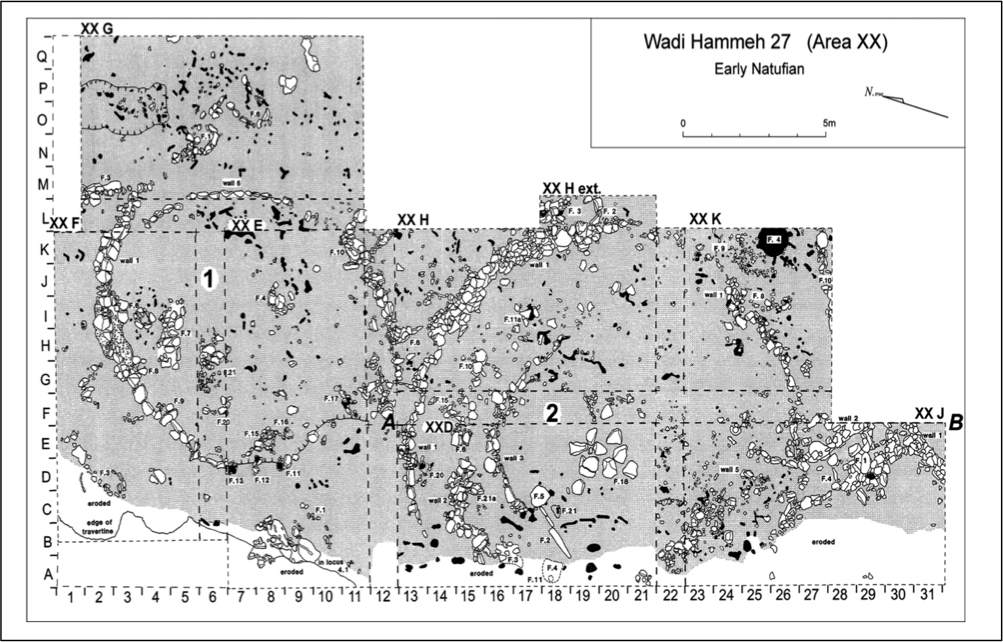
\includegraphics[width=\linewidth]{Gyngell-Fig01}
\caption{Plan of Wadi Hammeh 27, Phase 1.
        {\normalfont\scriptsize \\ \copyright\ by 
                 %\shortauthor
                 % or NAME OF COPYRIGHT HOLDER
	 \textcite{Hardy-Smith_2004}.}}
\label{fig:Gyngell-Fig01}
\vspace*{.9\baselineskip}
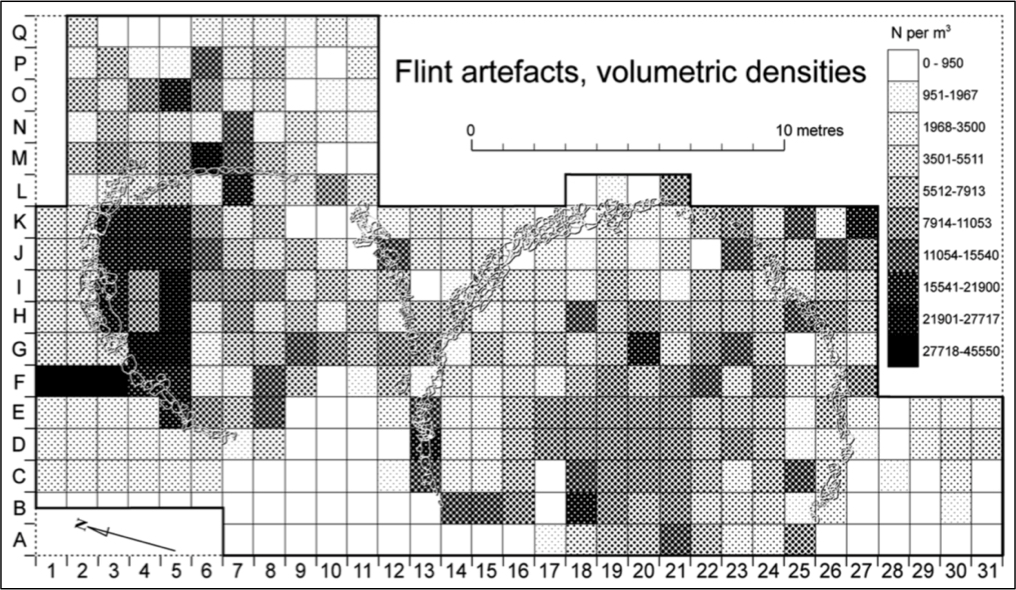
\includegraphics[width=\linewidth]{Gyngell-Fig02}
\caption{Volumetric distribution of flaked stone (flint) artefacts.
        {\normalfont\scriptsize \\ \copyright\ by 
                 %\shortauthor
                 % or NAME OF COPYRIGHT HOLDER
 \textcite{Hardy-Smith_2004}.}}
\label{fig:Gyngell-Fig02}
\vspace*{.9\baselineskip}
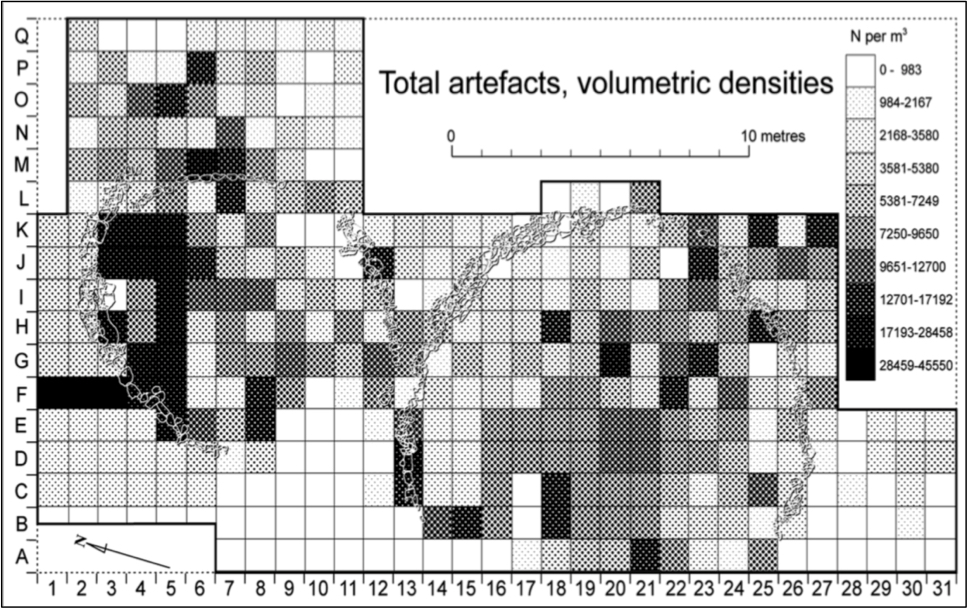
\includegraphics[width=\linewidth]{Gyngell-Fig03}
\caption{Volumetric densities of total artefacts.
        {\normalfont\scriptsize \\ \copyright\ by 
                 %\shortauthor
                 % or NAME OF COPYRIGHT HOLDER
 \textcite{Hardy-Smith_2004}.
                  }}
\label{fig:Gyngell-Fig03}
\end{wrapfigure}
\textcite[17--29]{Edwards_1989} continues to emphasise the complications of using settlement size and monumentality as a determinant for sedentism. 
He demonstrates the subjectivity of its nature and the capacity of large mobile groups to occupy sites that are similar to small sedentary occupations. 
% \parencite[17]{Edwards_1989}. 
The failure of many archaeologists to recognise the full capabilities of mobile peoples has led to exaggerated interpretations of sites and structures.
% \parencite[17]{Edwards_1989}. 
He firmly argues that mobile communities ‘have the time, capacity, organisational ability, and labour reserves to make large constructions,’ and demonstrates this using numerous ethnographic and prehistoric examples. 
%\parencite[17]{Edwards_1989}. 
The trend of underestimating mobile communities similarly led to the belief that Natufian storage facilities indicate sedentism.
% \parencite[25]{Edwards_1989}. 
%\textcite[25]{Edwards_1989} 
\citeauthor{Edwards_1989} 
argued that this is a result of the misconception that food stores must be guarded permanently. 
Finally 
%\textcite[29]{Edwards_1989} 
\citeauthor{Edwards_1989}
recognised the potential of analysing seasonality data. 
However, unlike the interpretations discussed above, 
%\textcite[29]{Edwards_1989} 
\citeauthor{Edwards_1989}
argues the evidence validates a reconstruction of Natufian semi-mobility. Therefore, it is clear that the Natufian debate has been dominated by miscalculated perceptions of mobile communities and sedentism that led to the ambiguous nature of the debate.

More recently, \textcite{Hardy-Smith_2004} conducted analysis on discard patterns and refuse behaviour at Wadi Hammeh 27 to demonstrate that the Natufian assemblage does not indicate that rubbish strategies required for sedentary living had been developed. 
This discussion is supported by \textcite{Fletcher_2007} argument that several material prerequisites are necessary in a cultural assemblage before communities are capable of sustaining sedentary settlements. 
\textcite[253]{Hardy-Smith_2004} systematically analysed artefact distributions and densities in and around two curvi-linear stone structures, interpreted as modest huts (\cref{fig:Gyngell-Fig01}).

They support their argument by providing explicit definitions of concepts including primary and secondary refuse \parencite[255]{Hardy-Smith_2004}. 
Nearly half a million artefacts were recorded in the huts, including flint and bone tools, basalt features, ochre fragments, and faunal and human remains \parencite[279]{Hardy-Smith_2004}. 
As the volumetric and areal density charts demonstrate, there is some indication of activity areas for stone tool manufacturing (\cref{fig:Gyngell-Fig02}). However, spatial organisation is not as extensive as the sedentary Neolithic structures, with no evidence of specialised craft made by regulated labour \parencite[282]{Hardy-Smith_2004}. 


Most significantly, \SI{82}{\percent} of artefacts were primary refuse clusters discarded within the dwellings \parencite[279]{Hardy-Smith_2004}, with very low indication of secondary refuse outside of the structures (\cref{fig:Gyngell-Fig03}). 
Therefore, the finds at WH27 indicate that the inhabitants lived on top of their garbage and reflect short-term settlements of a mobile community \parencite[285]{Hardy-Smith_2004}. 
\textcite[259]{Hardy-Smith_2004} also argue that WH 27 was deliberately abandoned and reoccupied, indicated by the regular reconstruction of walls and stone features. Thus, rigorous methodology and analysis of refuse disposal practices demonstrate that the Natufian assemblage is indicative of a mobile community.


\IJSRAsubsection{Strontium Isotope Analysis}
The application of strontium isotope analysis by \textcite{Shewan_2004} significantly advanced the understanding of Natufian assemblages, and demonstrated the potential for future research to combine with geological and chemical analysis.
Similarly to Edwards, \textcite[55]{Shewan_2004} recognised the problems caused by ambiguous definitions and the lack of thorough analysis of data within the debate. 
She supported Edwards’ argument that there are ‘no secure grounds to claim sedentism based on cultural markers’ \parencite[57]{Shewan_2004}. Consequently, Shewan aimed to provide an independent system to differentiate clearly between mobile and sedentary behaviour in the landscape. 
Strontium isotope analysis is a tool that Shewan used to compare strontium isotope ratios in animal and human bones, which reflects movement in the landscape \parencite[59]{Shewan_2004}. 
Species that regularly move around the landscape will demonstrate a wider variability of isotopic determinations, reflecting more geological formations \parencite[61]{Shewan_2004}. 
Therefore, \textcite[62]{Shewan_2004} obtained the strontium isotope ratios from several areas in the Levant (\cref{fig:Gyngell-Fig04}) to compare with the Natufian skeletal samples (\cref{fig:Gyngell-Fig05}). 

%\begin{wrapfigure}{O}[3cm]{0.5\textwidth} 
\begin{figure}[!b]
        \begin{subfigure}[t]{0.65\textwidth}
	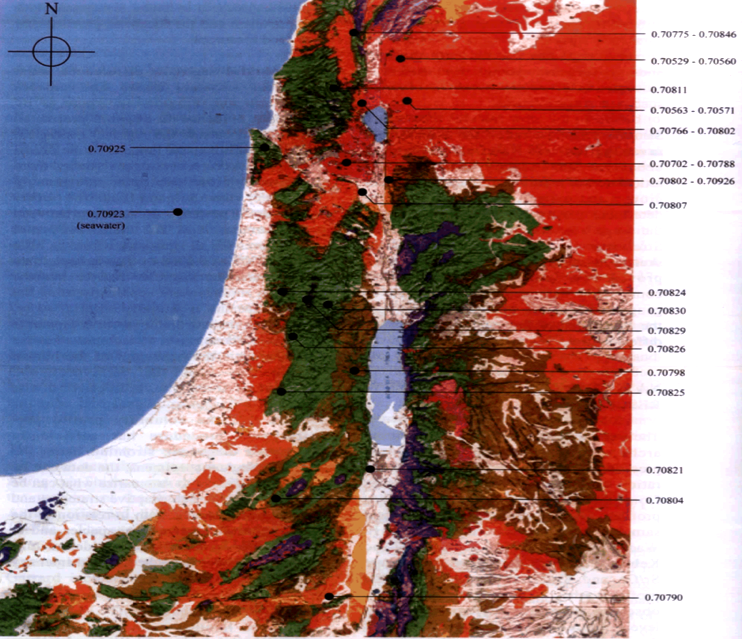
\includegraphics[width=\linewidth]{Gyngell-Fig04}
\caption{Measurements of strontium isotope ratios from modern fauna to demonstrate geological variation across the landscape, to compare with archaeological biologic samples.
        {\normalfont\scriptsize \\ \copyright\ by \textcite{Shewan_2004}.}}
\label{fig:Gyngell-Fig04}%
\end{subfigure}~
%\vspace*{.9\baselineskip}
\hspace*{1em}~\begin{subfigure}[t]{0.65\textwidth}
	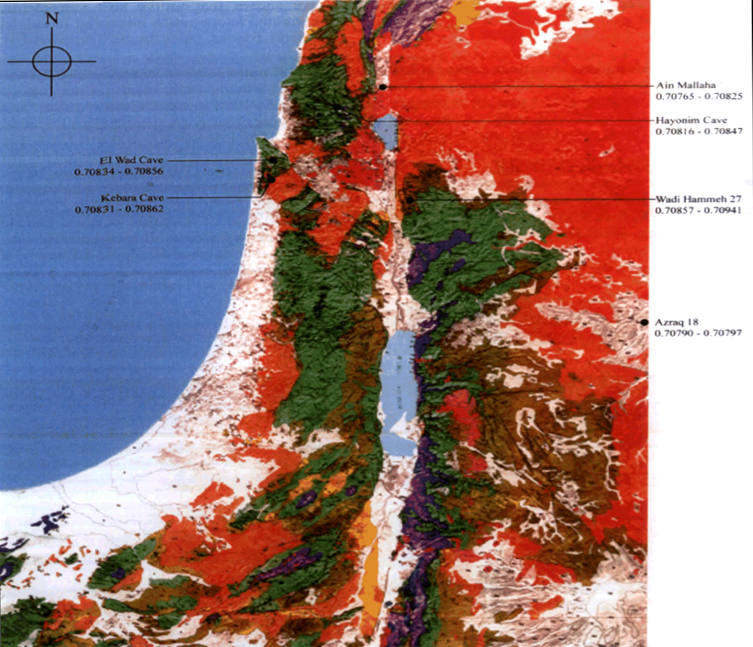
\includegraphics[width=\linewidth]{Gyngell-Fig05}
	
\caption{Strontium ratios in skeletal remains at Natufian sites.
        {\normalfont\scriptsize \\ \copyright\ by \textcite{Shewan_2004}.}}
\label{fig:Gyngell-Fig05}
\end{subfigure}
\caption{Measurements of strontium isotope ratios}
\end{figure}

Natufian sites included El Wad, Mt Carmel, Ain Mallaha and Wadi Hammeh 27. \textcite[71]{Shewan_2004} analysed the strontium isotope markers on human, gazelle and carnivore bones.

The results demonstrated the remarkable similarities between the specimens, thus reflecting the similar movement and behaviour of humans and animals in the Natufian landscape \parencite[79]{Shewan_2004} (\cref{fig:Gyngell-Fig06}). 
This study is very significant in the Natufian debate, as it does not rely on observations that are readily open to subjectivity. Although presentation of data is always at risk of manipulation, Shewan’s analysis encompasses numerous quantitative results collected using an explicit methodology and scientific techniques. 
Her use of geological and chemical principles in an archaeological context should be highly regarded for advancing the discussion, and should provide pathways for future study. 
Thus, \textcite{Shewan_2004} was able to demonstrate the mobile behaviour of the inhabitants of the Natufian landscape reflected in skeletal remains.
\clearpage
\IJSRAsubsection{New Research}
\begin{wrapfigure}{O}[3cm]{0.5\textwidth} 
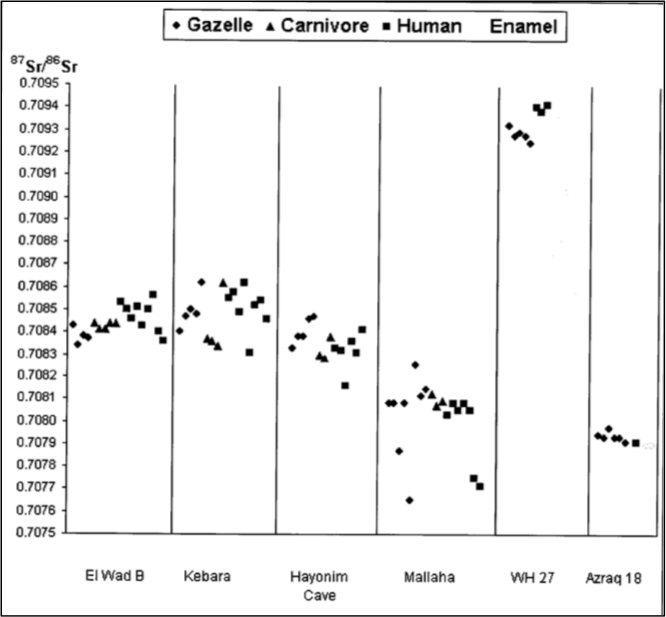
\includegraphics[width=\linewidth]{Gyngell-Fig06}
\caption{Strontium ratios in gazelle, carnivore and human bones at Natufian sites.
        {\normalfont\scriptsize \\ \copyright\ by 
                 %\shortauthor
                 % or NAME OF COPYRIGHT HOLDER
 \textcite{Shewan_2004}.
                  }}
\label{fig:Gyngell-Fig06}
\vspace*{.9\baselineskip}

	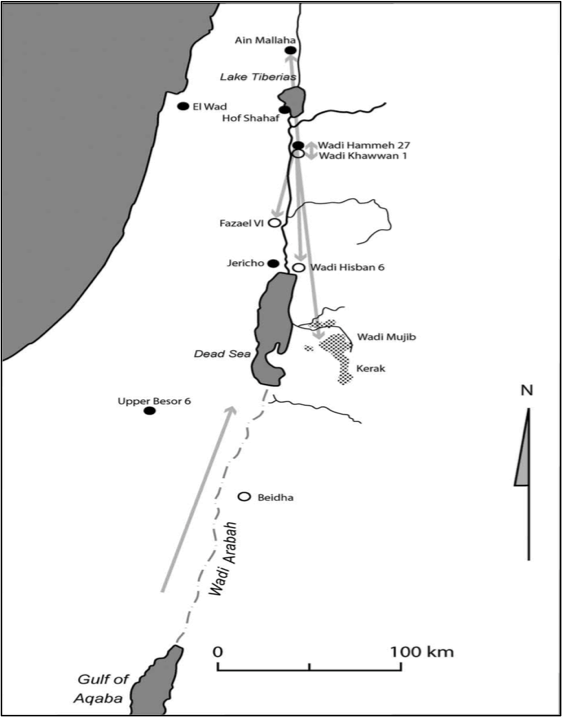
\includegraphics[width=\linewidth]{Gyngell-Fig07}
	\caption{Map indicating interaction zone and potential connections between Early Natufian sites.
		{\normalfont\scriptsize \\ \copyright\ by 
			%\shortauthor
			% or NAME OF COPYRIGHT HOLDER
			 \textcite{Edwards_2015}.
		}}
		\label{fig:Gyngell-Fig07}
\end{wrapfigure}

In the last decade research has been undertaken to study behaviour and interactions reflected in Natufian assemblages using a range of techniques. \textcite{Parslow_2009} implemented geographical information science (GIS) methods to argue that people were not constrained by environmental controls, and that groups interacted and shared technology. 
\textcite[3]{Parslow_2009} developed an interactive agency model to take account of human agency, and several spheres of interaction within and between groups at Natufian sites. 
\textcite{Edwards_2015}, building on a study by \textcite{Belfer-Cohen_2013}, similarly proposed a zone of interaction in the Early Natufian between open-air sites (\cref{fig:Gyngell-Fig07}). 
\textcite[547]{Belfer-Cohen_2013} critiqued past models that divide the Levant into a core and periphery area, which has prevented the study of regional variability. 
They demonstrated evidence of shared artefact styles between sites \textcite[546]{Belfer-Cohen_2013}. 
\textcite[272]{Edwards_2015} extended this argument by offering more examples of possible connections. 
\textcite[276]{Edwards_2015} proposed that stylistic traits are shared between WH27, Ain Mallaha and Fazael VI, including bird motifs on bone and stone artefacts, and patterns of grooves and ridges on stone bowls. 
He argued these examples and many more can be used to indicate patterns of Natufian settlement and interaction \parencite[280]{Edwards_2015}. Future scientific analysis of the artefacts and context will be fundamental for developing this model. However, it is an interesting new aspect to the debate.

\IJSRAsection{Future Debate}
The Natufian debate is hampered by the problem of defining sedentism. Numerous scholars recognised this issue, and attempted to move the debate in new directions by outlining the misleading assumptions and ambiguity that characterised early discussion. This problem is not symptomatic of the Natufian alone. 
\textcite{Habu_1996} demonstrated the tendency of scholars to assume that the prehistoric Japanese culture, the Jomon, occupied permanent camps year-round due to misunderstandings of what justifies sedentism. Future study of settlement behaviour reflected in Natufian assemblages and other transitional periods should firmly address this issue to remedy past misconceptions and enable substantial reconstructions. 
\textcite{Fletcher_2007} quantitatively addressed this issue and demonstrated that the transition from mobility to sedentism occurred after a number of prerequisites have developed. 
For example, \textcite{Fletcher_2007} argued that societies are not capable of occupying a settlement on a sedentary basis until they have begun building recti-linear structures. This is due to the need for predictable and regular space in sedentary settlements, which cannot be created using curvi-linear architecture typical of mobile communities. The interaction and communication demands of sedentism on communities are high and need to be regulated using a different settlement structure. This premise can be used to guide future research. 
The change from curvi-linear to recti-linear architecture, along with an increase in the number of rooms and a decrease in room size, is visible in the archaeological record \parencite{Byrd_2005}. An analysis of when and over what timeframe these changes occur will enable a quantifiable assessment of the transition from mobility to sedentism and provide a greater understanding of the Natufian assemblage.

The debate surrounding the Natufian began with heavily preconceived notions of sedentism and agriculture. Despite impressive archaeological excavation conducted by Bar-Yosef and other Near Eastern scholars, analysis of the data was inadequate to provide justifiable conclusions, and vague notions of sedentary lifeways impeded the discussion. Edwards demonstrated the inaccuracy of using cultural markers to claim Natufian sedentism, and instead claimed Natufian mobility using numerous examples of prehistoric mobile communities and ethnographic studies similar to the Natufian assemblage. Furthermore, rigorous methodology and scientific analysis conducted by Edwards and Shewan proved critical to the debate, demonstrating the mobile nature of people in the Natufian landscape and their incapability to sustain sedentary settlements. Future research should continue to critically analyse the Natufian assemblage and data, using a combination of disciplines and techniques, to develop a greater understanding of Natufian settlement patterns.

\IJSRAseparator
\IJSRAsection{Acknowledgements}
Many thanks to Roland Fletcher for advising me on my essay. 
Permissions to reprint images granted by Phillip Edwards and Tania Hardy-Smith.
\IJSRAclosing%<---- don’t change this!
%\end{document}